\documentclass[paper=a4, fontsize=11pt,twoside]{article}

% -------------------------------------------------------------------- 
% General Page Layout
% --------------------------------------------------------------------
\usepackage[a4paper]{geometry} 
\usepackage[parfill]{parskip}
\setlength{\oddsidemargin}{5mm}  % Remove 'twosided' indentation
\setlength{\evensidemargin}{5mm}

% --------------------------------------------------------------------
% Encoding and Language Settings
% --------------------------------------------------------------------
\usepackage[T1]{fontenc} 
\usepackage[utf8]{inputenc}   
% encoding may need to be changed depending on the system
\usepackage[swedish]{babel} 
\usepackage{lipsum} % Lorem Ipsum

% --------------------------------------------------------------------
%  Utilities (colors, links, pictures, ect...)
% --------------------------------------------------------------------
\usepackage{xcolor}
\usepackage{hyperref}
\usepackage{graphicx}
\usepackage{amssymb}
\usepackage{epstopdf}
\usepackage[round]{natbib}
\usepackage{float}
\usepackage{pgfplots}
\pgfplotsset{width=12cm,compat=1.9}
\usepackage{tikz}
\DeclareGraphicsRule{.tif}{png}{.png}{`convert #1 `dirname #1`/`basename #1 .tif`.png}

% -----------------------------------------------------------------------------%
% Title Page / Document Class Definitions (Please Don't Play With This)
% -----------------------------------------------------------------------------%
	
% Table of contents depth = section & subsection
\setcounter{tocdepth}{1}
																								
% Horizontal rule
\newcommand{\HRule}[1]{\rule{\linewidth}{#1}}   															
																											
% Document Number
\newcommand{\documentNumber}[1]{\centering PUSP1742#1 \\[1.0cm]}	 										
																											
% Document Version
\newcommand{\documentVersion}[1]{\centering \small{v.#1} \\[1.0cm]}

% Group Responsible
\newcommand{\documentResponsible}[1]{\centering  Ansvarig Grupp: #1}

% Document Creator Group
\newcommand{\documentCreator}[1]{\centering Uppgjord Av: #1}	 									
																										
% Title
\makeatletter \def\printtitle{ {\centering \@title\par}} \makeatother
																											
% Author .. not really used, but it can stay in case
\makeatletter \def\printauthor{ {\centering \large \@author}} \makeatother
																											
\newcommand{\grouptitlepage}[4]{ 
	\title{
		\documentNumber{#1}																						
		\documentVersion{#2}																				
		\HRule{0.5pt} \\ % Upper rule 
		\LARGE \textbf{\uppercase{#3}} \\
		\large \textbf{\uppercase{ETSF20 Grupp 2}} 
		\HRule{2pt} \\ [1.5cm]    
		\normalsize            
		\documentResponsible{#4} \\ 
		\documentCreator{#4}  
	}																							
	\maketitle																							
	\thispagestyle{empty} 																					
	\newpage 
}
% \grouptitlepage{doc number}{Version Number}{doc title}{group responsible for
% doc}
% --------------------------------------------------------------------------------%
% Title Page / Document Class Definitions (Please Don't Play With This)
% --------------------------------------------------------------------------------%


% \date{}                                            
% Activate to display a given date or keep commented for current date


% -------------------------------------------------------
% DOCUMENT START (YOU CAN IGNORE EVERYTHING ABOVE HERE)
% -------------------------------------------------------
\begin{document}

% -------------------------------------------------------
% Title Page START
% -------------------------------------------------------
\grouptitlepage
% the \# typesets a # character into the document, you will need to replace them
% in yourdocuments. This is a template, just plug in what you need between the
% {}s. Document Code Number (same as time reports)
{19}
% Document Version Number
{1.0}
% Document Title
{Projektslutrapport}
% Group Responsible For Document
{(PG) Projekt Grupp}
% -------------------------------------------------------
% Title Page END
% -------------------------------------------------------
\tableofcontents
% WRITE THINGS BELOW HERE

\section{Executiv summering}
En projektgrupp har utvecklat ett tidsrapporteringsystem inom ramarna för 
Pusp-kursen mellan den 16/1 och 23/3. Projektets slutprodukt fyller användarens 
krav och är lätt att använda. Dock så har projektgruppen haft svårt att
fullständigt följa vattenfallsprocessen och sk ”hjältar” har uppstått. 
Förbättringsrekommendationerna kretsar kring vikten av att arbete sker i 
gemensamma utrymmen och att tydligt diskutera målet med kursen.
\section{Inledning}
Detta dokument är en slutrapport av projektet som utvecklar
tidsrapporteringssystemet e-kyss.
\section{Projektets mål och begränsningar}
E-kyss har utvecklats av sexton studenter vid Lunds tekniska högskola för kursen 
”Programvaruutveckling för stora projekt”. Målet har varit att utveckla ett 
tidsrapporteringssystem med en väldokumenterad process och slutprodukt. 
Inom detta fanns särskilda mål för systemet och projektet separat; Systemet 
skulle vara webbaserat och uppfylla en mängd krav som kunden på förhand definierat. 
Medans projektet skulle följa vattenfallsmodellen som utvecklingsprocess.
Det övergripande målet för den omgivande kursen var att lära oss projektmetodik, 
samarbete och kommunikation vid utveckling i större grupper.\\
\\
Projektet inleddes tillsammans med kursen den 16/1-17 och avslutas den 23/3-17.
\newpage
\section{Refererade projektdokument}
\begin{figure}[h!]
\centering
\begin{tabular}{|l|c|c|c|}
\hline
Utvecklingsplan & PUSP174211 & v1.0 & SDP\\
\hline
Kravspecifikation & PUSP174212 & v1.2 & SRS\\
\hline
Testspecifikation & PUSP174213 & v1.0 & SVVS\\
\hline 
Högnivådesign & PUSP174214 & v1.0 & STLDD\\ 
\hline
Testinstruktion & PUSP174215 & v1.0 & SVVI\\
\hline
Lågnivådesign & PUSP174216 & v0.7?? & SDDD\\
\hline
Testrapport & PUSP174217 & v0.1 & SVVR\\
\hline
Systemspecifikation & PUSP174218 & v0.1 & SSD\\
\hline
\end{tabular}
\end{figure}

\section{Beskrivning av processen}
Vid projektgruppens första möte formerades ansvarsområden och arbetsgrupper. 
De grupper som skapades var Projektledare (PG) med två medlemmar, Systemansvariga (SG) 
med tre medlemmar, Utvecklare (UG) med åtta medlemmar och Testare (TG) med tre
medlemmar.\\
\\
Efter detta möte ansågs projektets första fas av fyra påbörjad. 
(Se ”Projekthanledning” v2.3 för beskrivning av vattenfallsmodellen och dess faser.)
Under den första veckan skapades en planering som kom att ligga till grund för 
projektgruppens arbete. Denna finns i detalj i projektdokumentet SDP men kommer här att 
summeras med kommentarer och jämförelser med verkligt utfall.
Den ursprungliga planeringen skapades med ambitionerna att arbetsbördan inte skulle 
överstiga tio timmar per person och vecka, att arbete i huvudsak skulle ske mellan klockan 
åtta och fem under veckodagar och att veckor där andra kurser tog upp mer än trettio 
timmar flyttades arbetstid till veckor där detta inte var fallet.
Skattningar på förväntat tidsåtgång av faser och dokument var en viktig del av 
planeringen, men då ingen av projektmedlemmarna arbetat på ett liknande sätt tidigare 
baserades dessa skattningar på litteratur om vad som är vanligt inom arbetslivet. Kort 
sagt gjordes dessa med stor förväntad felmarginal.

\begin{table}[H]
\centering
\caption{Planerade datum:}
\begin{tabular}{| l | c | c | c | c |} %5
\hline
 & Fas 1 & Fas 2 & Fas 3 & Fas 4\\
\hline
Start: & v3 & v6 & v8 & v10 \\
\hline
Stopp: & v6 & v8 & v11 & v12 \\
\hline
 				& SDP & & & PFR \\
Dokument: & SRS & STLDD & SDDD & SSD \\
 				& SVVS & SVVI & & SVVR \\
\hline
InfGran: & 30/1 & 17/2 & 15/3 & 	 \\
\hline
FormGran: & 6/2 & 22/2 &	 & 23/3 \\
\hline
OmGran: & 10/2 & 1/3 &		 & \\
\hline
\end{tabular}
\end{table}

\begin{table}[H]
\centering
\caption{Skattad tidsåtgång:}
\vspace{0.2cm}
\begin{tabular}{| l | c | c | c | c | c | c | c | c | c | c |}
\hline
 & \textbf{v3} & \textbf{v4} & \textbf{v5} & \textbf{v6} & \textbf{v7} & \textbf{v8} & \textbf{v9} & \textbf{v10} & \textbf{v11} & \textbf{v12}\\
\hline
\textbf{Arbetstid:}  &  & 8 & 6 & 16 & 14 & 26 & 22 & 20 & 24 & 18 \\
\hline
\end{tabular}
\end{table}

\begin{figure}[h!]
\centering
\caption{Faktiska värden:}
\begin{tabular}{|l|c|c|c|c|c|}
\hline
\textbf{Dokument} & {\fontsize{8pt}{0.2cm}\selectfont Total} &
{\fontsize{8pt}{0.2cm}\selectfont Utveckling} &
{\fontsize{8pt}{0.2cm}\selectfont Informell Granskning} &
{\fontsize{8pt}{0.2cm}\selectfont Formell Granskning} &
{\fontsize{8pt}{0.2cm}\selectfont Omarbete}\\
\hline
SDP & 72.0 & 52.0 & 2.0 & 5.6 & 12.4\\
\hline
SRS & 138.3 & 111.6 & 8.5 & 6.0 & 12.3\\
\hline
SVVS & 54.5 & 36.7 & 5.2 & 7.2 & 5.5\\
\hline
STLDD & 224.0 & 205.4 & 7.2 & 5.6 & 6.0\\
\hline
SVVI & 38.3 & 29.9 & 5.0 & 1.4 & 2.0\\
\hline
SDDD & 129.3 & 129.3 & - & - & -\\
\hline
SVVR & 10.8 & 10.8 & - & - & -\\
\hline
SSD & 69.3 & 69.3 & - & - & -\\
\hline
PFR & 23.4 & 23.4 & - & - & -\\
\hline
\end{tabular}
\end{figure}

\begin{figure}[h!]
\centering
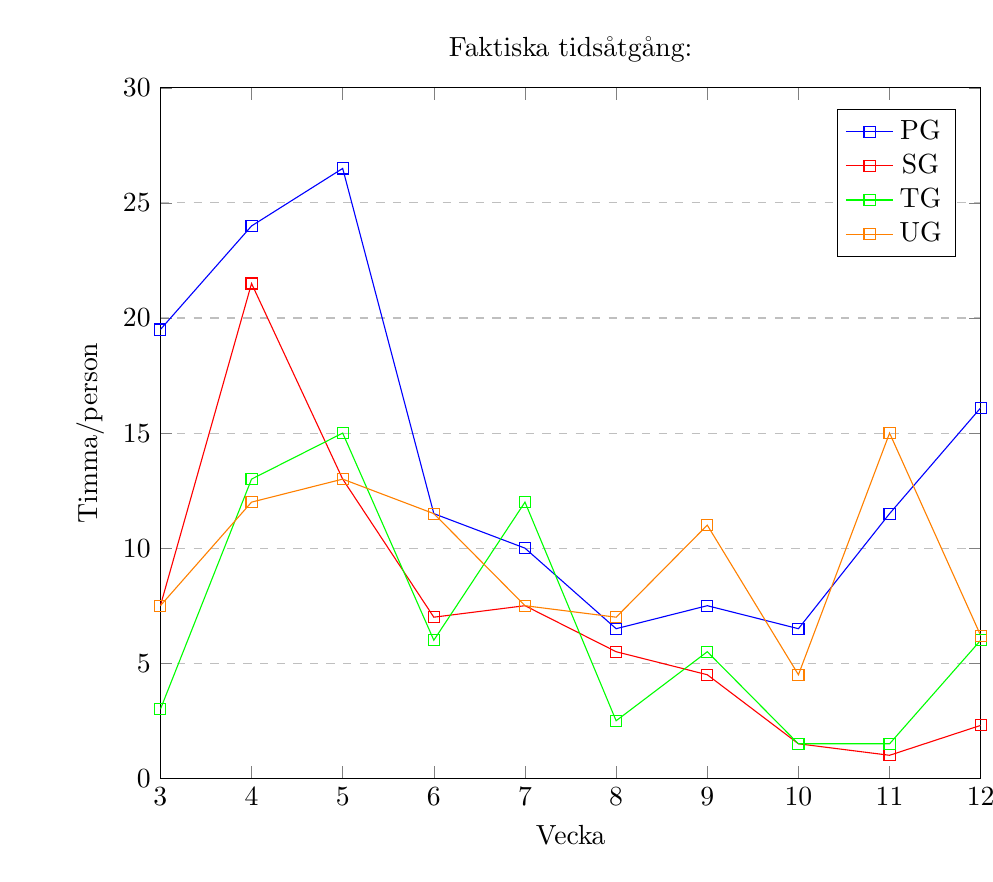
\begin{tikzpicture}
\begin{axis}[
    title={Faktiska tidsåtgång:},
    xlabel={Vecka},
    ylabel={Timma/person},
    xmin=3, xmax=12,
    ymin=0, ymax=30,
    xtick={3,4,5,6,7,8,9,10,11,12},
    ytick={0,5,10,15,20,25,30},
    legend pos=north east,
    ymajorgrids=true,
    grid style=dashed,
]
%PG

\addplot[
    color=blue,
    mark=square,
    ]
    coordinates {
    (3,19.5)(4,24)(5,26.5)(6,11.5)(7,10)(8,6.5)(9,7.5)(10,6.5)(11,11.5)(12,16.1)
    };
%\addplot[color=blue]{14};

%SG 
\addplot[
    color=red,
    mark=square,
    ]
    coordinates {
    (3,7.5)(4,21.5)(5,13)(6,7)(7,7.5)(8,5.5)(9,4.5)(10,1.5)(11,1.0)(12,2.3)
    };
%\addplot[color=red]{7.2};

%TG
\addplot[
    color=green,
    mark=square,
    ]
    coordinates {
    (3,3)(4,13)(5,15)(6,6)(7,12)(8,2.5)(9,5.5)(10,1.5)(11,1.5)(12,6)
    };
%\addplot[color=green]{6.6};

%UG
\addplot[
    color=orange,
    mark=square,
    ]
    coordinates {
    (3,7.5)(4,12)(5,13)(6,11.5)(7,7.5)(8,7)(9,11)(10,4.5)(11,15)(12,6.2)
    };
%\addplot[color=orange]{10.1};
\legend{PG,SG,TG,UG}
 
\end{axis}
\end{tikzpicture}
\caption{Genomsnitt arbetstid per gruppmedlem.}
\end{figure}

\begin{itemize}
  \item fas 1: v3 – v10 arbete skedde ej aktivt efter v8
  \begin{enumerate}
    \item 16/1 - Start v3
    \item 1/2 - informell v5
    \item 6/2 - Gransking 1 v6
  \end{enumerate}
  \item fas 2: v6 – v10
  \begin{enumerate}
    \item 18/2 - inställd informell granskning fas 2, blev möte istället v7 23/2 
    \item Sista insändning av fas 1 v8 
    \item 1/3 - Insändning fas 2 v9 
    \item 6/3 - Granskning 2 v10
  \end{enumerate}
  \item fas 3: v10 – v12
  \begin{enumerate}
    \item 10/3-14/3 tentaperiod v10-v11 
    \item Därefter en galen rush att möta deadlinen v12
  \end{enumerate}
  \item fas 4: v11 - v12
\end{itemize}

Möten var 13 planerade och ca 12 genomfördes. \\

\begin{figure}[h]
\centering
\caption{Arbetsfördelning över gruppmedlem:}
\begin{tabular}{|l|c|c|c|c|c|c|c|c|c|c|c|}
\hline
{\fontsize{8pt}{0.2cm}\selectfont stil\_id} & {\fontsize{8pt}{0.2cm}\selectfont
total} & {\fontsize{8pt}{0.2cm}\selectfont v.3} &
{\fontsize{8pt}{0.2cm}\selectfont v.4} & {\fontsize{8pt}{0.2cm}\selectfont v.5}
& {\fontsize{8pt}{0.2cm}\selectfont v.6} & {\fontsize{8pt}{0.2cm}\selectfont v.7}
& {\fontsize{8pt}{0.2cm}\selectfont v.8} & {\fontsize{8pt}{0.2cm}\selectfont v.9}
& {\fontsize{8pt}{0.2cm}\selectfont v.10} & {\fontsize{8pt}{0.2cm}\selectfont
v.11} & {\fontsize{8pt}{0.2cm}\selectfont v.12} \\
\hline
dat13mde & 5485 & 720 & 1470 & 840 & 640 & 720 & 405 & 390 & 120 & 180 & - \\
\hline
dat14sfa & 8970 & 680 & 750 & 1265 & 760 & 510 & 575 & 1500 & 255 & 2475 & 200
\\
\hline
dat15bho & 4160 & 315 & 1210 & 885 & 345 & 360 & 420 & 330 & 90 & 145 & 60 \\
\hline
dat15cri & 3340 & 310 & 1150 & 590 & 285 & 285 & 165 & 120 & 45 & 45 & 345 \\
\hline
dat15csh & 5680 & 480 & 730 & 1065 & 765 & 645 & 525 & 420 & 150 & 450 & 450 \\
\hline
dat15jsu & 9065 & 365 & 940 & 750 & 1100 & 660 & 430 & 935 & 375 & 2640 & 870 \\
\hline
dat15mga & 3750 & 375 & 575 & 360 & 450 & 310 & 300 & 420 & 60 & 600 & 300 \\
\hline
dat15rel & 2425 & 360 & 405 & 420 & 410 & - & 300 & 430 & 100 & - & - \\
\hline
dat15sbe & 2970 & 345 & 445 & 525 & 330 & 330 & 300 & 270 & 240 & 185 & - \\
\hline
elt13spl & 2655 & - & 645 & 555 & 180 & 600 & 150 & 375 & 150 & - & - \\
\hline
fte11ama & 6630 & 710 & 965 & 1375 & 710 & 340 & 320 & 225 & 540 & 535 & 910 \\
\hline
gda10apo & 11367 & 450 & 1460 & 1222 & 1290 & 690 & 600 & 1740 & 255 & 2520 &
1140
\\
\hline
gin10ekr & 4520 & 295 & 1290 & 990 & 465 & 810 & 90 & 315 & 100 & - & 165 \\
\hline
mat13cgu & 4200 & 525 & 375 & 565 & 375 & 350 & 240 & 360 & 150 & 1260 & - \\
\hline
nat14ero & 4760 & 295 & 390 & 1120 & 455 & 755 & 210 & 320 & 55 & 250 & 910 \\
\hline
sas10gau & 10065 & 1635 & 1935 & 1790 & 660 & 840 & 470 & 640 & 245 & 825 &
1025 \\
\hline
\end{tabular}
\end{figure}


Att planeringen och utfallet gått isär är lätt att se:
\begin{itemize}
  \item Fas 1 gick officiellt sett inte i baseline innan v10, men var då klar sedan ett par veckor.
  \item Fas 2 är tydligt en av de största förseningarna i projektet vilket tillsammans med en alltför generös tentamensperiod skapade en sammansatt fas 3 och 4.
\end{itemize}
Förseningen vid denna fas orsakades av att arbetet runt högnivådesignen var oorganiserat. 
I brist på tydligt ansvar för översikt fylldes dokumentet med irrelevant och felaktigt arbete. 
När väl problematiken uppdagades låstes dokumentet och omformaterades
grundligt.\\
Ett av projektets största utmaningar planeringsmässigt var att alla projektmedlemmar 
kan liknas vid deltidsanställda. Att arbetstid har planerats allteftersom det fanns 
plats på schemat har skapat tidsmässig fragmentering och en avsaknad av rutin. Detta har 
i sin tur tillsammans med den varierande arbetsbördan skapat en ytterligare rumslig 
fragmentering av projektgruppen. Alltför lite tid har spenderats i samma rum där man enkelt 
kunde kommunicera och samarbeta.\\
I utvecklingsplanen ingick även specifiseringar av vilka metoder, tekniker och hjälpmedel 
som skulle användas samt vilka regler som skulle gälla för arbetet.\\
Av alla dessa är det värt att nämna de som antingen påverkat arbetet stort 
eller som helt frångåtts:
\begin{itemize}
  \item HTML användes inte explicit som beskrivs. Istället har JSP (JavaServer
  Pages) används. Dessa genererar i sin tur HTML.
  \item Att Eclipse skulle användas frångicks under sista veckorna. Detta då
  mycket kod redan skapats med Intellij istället och det blev enklare än att 
  omforma projektfilerna för Eclipse.
  \item Projektbiblioteket har genomgått ett flertal faser. Vid ett flertal
  tillfällen har det blivit oöverskådligt då det används felaktigt med versioner 
  och tillägg som lades till på olika och inkonsekventa sätt.
  \item Regeln att inte förvänta sig arbete utanför ”normal” arbetstid utgick i
  slutet på februari.
\end{itemize}

Slutligen så innehöll utvecklingsplanen även risker som vi förutsåg kunde komma 
att drabba projektet. Tursamt nog inföll de flesta inte, men det som vi i huvudsak 
drabbats av har varit brist på rätt kunskaper. Detta förvärrades av att vissa 
utvecklare inte heller använde det vedertagna IDE:t. De som redan var utmanade att 
förstå uppgiften i en miljö de var vana vid fick ytterligare en svårighet. Tiden 
som spenderades på att installera, förklara, förstå och lära sig intellij skapade 
extra arbete som kunde ha undvikits.

\section{Projektanalys}
Projektet har gått långt ifrån felfritt men flera av projektmedlemmarna har 
beskrivit en känsla av förtroende för att det kommer gå i hamn.

Det som projektgruppen upplever att den misslyckats med är i huvudsak att följa 
vattenfallsprocessens metodik och att uppnå en jämn arbetsfördelning mellan 
projektmedlemmarna. Vattenfallsprocessen signum är ansvarsfördelning och dokumentation 
som låter vitt skilda avdelningar och projektmedlemmar samarbeta med minimal 
kommunikation. Projektetgruppen har följt processmetodiken, men en klart förenklad 
version:
\begin{itemize}
  \item Informella granskningar var mycket informella.
  \item Baseline för fas 1 blev inte bekräftad förän fas 2 granskades formellt.
  \item Status och problemrapportering har varit bristfällig.
  \item Testprotokoll har varit svåra att upprätta.
\end{itemize}

Då fas 1 dokumenten gick i baseline samtidigt med de från fas 2 skapades få 
problemrapporter och förändringskontroll behövdes inte under de första faserna. 
Därigenom fick arbetsgruppen mycket lite erfarenhet att upprätta och underhålla 
status- och problemrapporter.

Under vad som blev den rätt gemensamma utvecklings och testningsfasen fick 
testare kämpa för att hålla ikapp med utvecklare som själva testade nogrannt 
och utan att uppföra testprotokoll åtgärdade fel och skapade nya beta-versioner. 
Tidvis så många som fem på ett dygn. Att detta tilläts fortlöpa under 
flera dagar var ett symptom av den extrema tidspress utvecklingsgruppen hamnade 
under i de sista två veckorna.

Tidspressen som uppstod hade sin orsak i en mängd av problem. Dels så försenades 
högnivådesignen med minst fem dagar men vi tog också fler dagar till 
tentamensförberedelser än vad vi hade råd med. I efterhand så är vansinnet uppenbart 
i att avsätta fem hela dagar till databastentamen när vi är så nära vår deadline. 
Men de oväntade goda vitsorden vi fått på granskningen av fas 2-dokumenten gjorde oss 
övermodiga.\\

Utvecklingsprocessen plågades också av fler problem inom kommunikation, 
verktygshantering och förkunskaper. Den tidigare nämda fragmenteringen i tid och 
geografi gjorde det svårt för utvecklarna att samordna vem som gjorde vad.\\

Ett oväntat byte av utvecklingsmiljö försvårade även det utvecklingsprocessen: 
De utvecklare som redan innan hade en mindre förståelse för systemets beroenden och 
struktur blev så tvungna att lära sig en ny arbetsmiljö.\\

Med det inte sagt att det var fel att byta eller att ansvaret ligger på de som 
förespråkade förändringen. Vid analys av inrapporterad arbetstid ses ett tydligt 
sammanhang mellan tiden investerad i fältet ”Hemstudier” och med produktiviteten 
vid slutet av projektet. Bytet av utvecklingsmiljö försvårade visserligen deltagande 
i utvecklingen men flera utan tidigare erfarenhet av den nya miljön tillhörde de mest 
produktiva givet att de tagit iniativ till hemstudier.\\

Det är ingen tvekan om att hjältar uppstått inom projektgruppen. 
Att så har skett är ytterst projektledarnas fel även om kommunikationen har 
varit bristfällig därom.\\

Kommunikationen och hur väl den fungerat har varit det mest centrala för projektet. 
Den har i stort fungerat väl, men det har räckt med små störningar för stora konsekvenser. 
Projektgruppen har användt sig i extremt hög grad av textchattar i programmet Discord för 
sin dagliga kommunikation. Att vi haft en regel som kräver att alla uppdaterar sig 
själva där minst en gång om dagen gjorde ofta möten som informationsverktyg överflödiga. 
Att små störningar gav stora konsekvenser kan vara en bieffekt av hur lätt man blev 
van att kunna komma åt andra och informationen man behövde. Vid bristande kommunikation 
uppstod problem såsom: oklarheter i ansvar och uppgifter, dubbelarbete och ojämn 
arbetsfördelning.\\

Arbetsfördelningen har både varit ojämn mellan personer men också över tid. 
Troligtvis ett vanligt problem inom vattenfallsmodellen, men grupper som har det 
tyngst mot slutet av projektet riskerar att betala ett högt pris för sina kollegors 
förseningar inom andra områden. Detta tillsammans med arbets-fragmentering skapade för 
vissa en mycket bristande känsla av gemenskap.\\

Trots många problem så har inga öppna konflikter uppstått. Trots allt så har många 
uppskattat arbetet då de upplever att de lärt sig mycket och då de har utökat sina 
sociala kontakter. Det som de flesta upplever sig nöjda med hur kommunikationen fungerat, 
effektiviteten vid dokumentskrivande och den goda tonen. Flera känner också en stolthet 
i systemet eller den dokumentation som skapats.\\

\section{Förbättringsförslag}
Skulle vi som projektgrupp börja om hela projektet på nytt så finns det en rad saker 
vi skulle vilja förbättra. Det kanske viktigaste skulle vara att tydligare utvärdera 
vår målsättning under projektet, det är lätt att få tunnelseende med fokus på just 
dokument och programmering. Men hade vi på förhand diskuterat och tydligt poängterat 
förbättringar inom kommunikation, samarbete och ansvarsfördelning som målsättning 
så hade vi troligtvis sett en mycket annorlunda process. Det vi skulle vilja uppnå 
med detta är en process som är mer fokuserad på processen i sig och lärande, snarare 
än på slutprodukten.\\

``Diskutera tidigt målet med kursen utöver projektet. Det handlar inte om att
lära sig programmera.''\\

För att förbättra problemen runt förlorad tid och den ojämna arbetsfördelningen
så skulle vi vilja lägga större vikt vid arbetstider. Värdet av att redan 
tidigt skapa en rutin där man tar för vana att sitta tillsammans skulle 
ha för oss jämnat ut arbetsfördelningen och förebyggt förseningar och
kunskapsbrist.\\

``Borde personligen lagt mer tid på förberedelser.''\\

Det är tydligt i projektgruppen att kommunikation upplevs som avgörande. 
Nästan alla förbättringar som föreslagits är på något sätt kopplad till just 
kommunikation.\\

Några av dessa förslag innefattar:
\begin{itemize}
  \item Var noga med att alla vet vilken utvecklingsmiljö som används.
  \item Se till att återkommande fråga hur det går till inviduella medlemmar.
  \item Använd voip i större utsträckning.
  \item Tillsätt en officiell ledare för utvecklingsgruppen.
\end{itemize}

\subsection{Vad har vi uppnått?}
Systemet som skapats under projektet uppfyller alla de formella kraven från kunden. 
Därtill har det en snygg och lätt användarupplevelse som fungerar på diverse 
webläsare och apparater.\\

Vi har lärt oss om Vattenfallmetodens arbetsmetodik och därigenom kommit att
uppskatta agila metoder.\\

Det kanske viktigaste är att vi har fått insikter om vikten av kommunikation, 
dokumentering och arbetsprocesser inom mjukvaruutveckling.\\

\subsection{Tack till}
Vi vill uttrycka vår tacksamhet till våra utomstående intressanter:
\begin{itemize}
  \item [] Sektionschefen Christin Lindholm för utbildning, stöd och
  handledning.
  \item [] Experten Anders Bruce för stöd och kunskap.
  \item [] Samt vår expert och granskare Alma Orucevic-Alagic för handlening,
  granskning och villighet att läsa våra dokument över helger.
\end{itemize}  
Tack.







\end{document}










